\chapter{EL PROBLEMA}
\label{capitulo1}

% De qué va a tratar el capítulo
% El capítulo 1 suele ser el marco teórico.
\section{Planteamiento del problema}

Internet con el pasar de los años se ha estado integrando cada vez más en varios aspectos de nuestras vidas. A pesar de todos los beneficios que trae estar tan conectados a esta red de redes, es preciso recalcar igualmente los problemas que acarrea el hecho de estar conectado a esta sin la existencia de medidas de seguridad necesarias. 

Los dispositivos, las aplicaciones y los sistemas que utilizamos en nuestro día a día almacenan información valiosa a la que pueden acceder personas no deseadas si no existen las medidas necesarias en las redes para evitar los ciberataques. Cada día más y más información digital existe en el mundo, y mientras crece el volumen de dicha información , aumenta también la cantidad de ciberataques que se realizan \cite{pwc}. Es por esta razón, que el concepto de ciberseguridad es de vital importancia cuando hablamos del cibermundo.  La ciberseguridad, se encarga de proteger redes de comunicación, sistemas y datos de ataques cibernéticos. 

Uno de los métodos utilizados en la ciberseguridad son los detectores de intrusiones (IDS, por sus siglas en inglés Intrusion-detection system). Un IDS es detector que procesa información proveniente del sistema o redes de computadores que se desea proteger. Una vez que que detectada una intrusión este lanza alertas para activar el proceso de auditoría por parte de los administradores de sistema \cite{IDS}. 

Por otra parte, uno de los servicios más utilizados en el mundo del Internet y que más contienen información son los servicios web. Estas características hacen que este tipo de servicios sea uno de los más apetecibles para los ciberataques. Se hace evidente entonces, que se requieren medidas en el área de la ciberseguridad dirigidas a estos casos.

Es por esta razón que grupos de investigación se han dedicado a tratar de solventar dicho problema. Tal es el caso del grupo de investigación de la Universidad de Granada que  ha desarrollado un IDS para detectar ataques a servidores web llamado SSM ("Segmented Stochastic Modelling") y así evitar problemas como: el reconocimiento, el escaneo de paquetes de red, la obtención y el mantenimiento de acceso al servidor y la modificacion de ``logs'' que evitan que se rastree el ataque en este tipo de servicios.

Es por ello que resultaría interesante implementar un sistema de intrusiones que ha presentados resultados satisfactorios como es el caso de SSM haciendo uso de una herramienta tan potente y en auge como lo es Bro.

\section{Objetivos}
\subsection{Objetivos generales}
El objetivo del presente trabajo es incorporar la técnica de detección de intrusiones SSM propuesta en \cite{ssm} en el sistema Bro. Para ello deben usarse las capacidades de scripting de Bro e incorporar las funcionalidades necesarias como un módulo que pueda activarse a demanda para monitorizar las peticiones a los servicios web.
\subsection{Objetivos específicos}
La consecución del objetivo general planteado puede abordarse a partir de los siguientes objetivos específicos:

\begin{enumerate}
\item Interceptar las URI para su análisis haciendo uso de Bro para capturar y filtrar la información de los paquetes del protocolo HTTP.
\item Desarrollar un módulo que permita evaluar el índice de anomalía de los URI haciendo uso de las herramientas otorgadas por el lenguaje de scripting de Bro y siguiendo las especificaciones y expresiones pautadas por la técnica de detección de intrusiones SSM. 
\item Desarrollar un módulo para la estimación de los modelos de normalidad haciendo uso de las herramientas otorgadas por el lenguaje de scripting de Bro que permita obtener un modelo de normalidad a partir de trafico libre de ataques.
\item Evaluar experimentalmente el funcionamiento del sistema realizando pruebas, tanto funcionales como operativas para verificar el correcto funcionamiento del mismo.
\end{enumerate}

\section{Justificación e importancia}


La intención del proyecto es implementar un detector de intrusiones para servicios web, basado en SSM haciendo uso de la herramiento Bro.

Un Detector de Intrusiones (IDS) es un sistema que monitoriza todas las actividades de un sistema en específico para detectar intrusiones\cite{IDSdef}. Si el mismo detecta una intrusión, se generará una alerta para que los administradores del sistema se encarguen de la misma.

Sin embargo, una pregunta válida que se puede realizar es : ¿Para qué molestarse en instalar un IDS si se tiene un ``firewall'', filtro de ``spam'' y contraseñas de autenticidad? La respuesta es simple: porque las intrusiones siguen ocurriendo. Así como las personas algunas veces olvidan cerrar las ventanas, por ejemplo, también olvidan actualizar el conjunto de reglas del ``firewall''. \cite{IDSimportance}

Es por esto, que los IDS conforman un aspecto importante dentro de la seguridad, ya que si alguno de los elementos fallan siempre estará el detector de intrusiones para generar alertas sobre posibles ataques.

Por otra parte, SSM es un sistema basado en el uso de modelos realizados a partir de las peticiones hechas al servicio web. Los resultados experimentales en este sistema muestran la eficacia del mismo detectando anomalías en este tipo de servicios. Sin embargo, la implementación disponible de SSM es de laboratorio y funciona sobre trazas estáticas, por lo que la técnica no está disponible actualmente para su uso en redes en explotación.

No obstante, para que realizar una implementación de sistema que funcione en redes en explotación, se requieren de herramientas aptas que permitan capturar y analizar el tráfico en la red. Por su parte, Bro, es un sistema de monitorización de red de código abierto muy utilizado hoy en día para el desarrollo de mecanismos de seguridad que posee: su propio lenguaje de scripting y una comunidad de asistencia que va creciendo cada vez más con el tiempo.

Por lo tanto, implementar una técnica que ha tenido resultados satisfactorios como lo es SSM, haciendo uso de Bro, que es una herramienta en auge en el ámbito de la seguridad de redes hoy en día resulta de mucha utilidad ya que esta unión permitirá de manera satisfactoria detectar intrusiones en los servicios web en producción para de esta manera alertar en la manera de los posible sobre ataques de reconocimiento, escaneo, la obtención y el mantenimiento de acceso al servidor y la modificación de ``logs'' que evitan que se rastree el ataque.


\section{Planificación}

La tareas en las que se divide el desarrollo de este proyecto fueron las siguientes:

\newlist{legal}{enumerate}{10}
\setlist[legal]{label*=\arabic*.}

\begin{legal}
\item Estado del arte

Durante esta etapa se realizará un estudio sobre los IDS, los tipos de IDS y el sistema SSM. Así mismo, se hará una lectura del RFC 3986 (URI) y se investigará sobre el protocolo HTTP.

\item Análisis de Bro

Durante esta etapa del proyecto se instalará, se estudiará la documentación y se aprenderá a hacer uso de la herramienta Bro y su lenguaje de scripting.

\item Arquitectura modular del sistema 

En esta etapa se realizará el diseño de los módulos principales que conforman el sistema. Esta tarea se basará en dividir el trabajo de cada uno de los módulos en varias funcionalidades y en diseñar las estructuras de datos y el formato de los archivos de texto del sistema.

    Esta tarea estará subdividida en las siguientes subtareas:

\begin{legal}
\item Diseño del módulo de análisis sintáctico/segmentación de URIS 
\item Diseño del módulo de evaluación de URIs 
\item Diseño del módulo de entrenamiento 
\end{legal}
\item Implementación del sistema

En esta etapa del proyecto se llevará a cabo la implementación del sistema haciendo uso del lenguaje de scripting de Bro.

\begin{legal}
\item Módulo de análisis sintáctico/segmentación de URIS 

En esta etapa se tomarán los diseños esbozados previamente y se implementarán todas las funcionalidades necesarias para realizar el segmentador y el analizador sintáctico de los URIS.

\item Módulo de evaluación de URIs 

En esta etapa  se implementarán todas las expresiones, las estructuras de datos y las funcionalidades necesarias para construir un modulo de evaluación funcional haciendo uso de las herramientas presentadas por Bro. 

\item Módulo de entrenamiento 

En esta etapa se implementarán las estructuras de datos y módulo de entrenamiento.

\item Módulo de gestión del tipo de sistema

En esta etapa del proyecto se implementará el módulo de gestión del tipo de sistema haciendo uso de "bash scripting". 

\item Módulo de reportes

En esta etapa se implementarán los reportes del sistema haciendo uso de herramientas de Bro dedicadas exclusivamente a realizar este tipo de tareas.

\end{legal}
\item Evaluación y pruebas 

Durante el desarrollo del proyecto se realizarán pruebas funcionales y una vez finalizada la implementación del sistema se procederá a realizar pruebas operativas.
\begin{legal}
\item Realización de pruebas funcionales

Se harán pruebas de manera individual a cada una de las funciones más importantes de los módulos que conforman el sistema y se realizarán las modificaciones pertinentes en las mismas.

\item Realización de pruebas operativas

La realización de las pruebas operativas se basará en tomar base de datos de trazas tanto normales como anormales, probar el funcionamiento de todo el sistema y realizar las modificaciones pertinentes.

\end{legal}

\item Documentación  
 Esta fase consistirá en estructurar y redactar la memoria del proyecto.
\end{legal}

\begin{figure}[tb]
\begin{center}
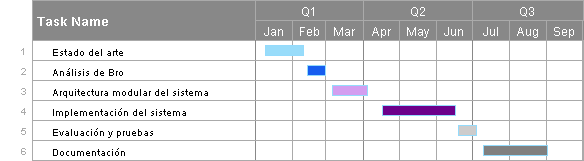
\includegraphics[width=4in]{Proyecto-grado.png}
\caption{Diagrama de Gantt del proyecto.}\label{fig1}
\end{center}
\end{figure}

